

\chapter{Warm core rings release predators from thermal constraints when foraging in the ocean Twilight zone}
\label{chap:5}
\raggedbottom

{\let\thefootnote\relax\footnotetext{This chapter was modified to short format and accepted for publication as Braun, C.D., Gaube P., Sinclair-Taylor T., Skomal, G.B., and Thorrold S.R. Warm core rings release predators from thermal constraints when foraging in the ocean Twilight zone. \emph{Journal name}. }}
%\end{singlespace}
{\let\thefootnote\relax\footnotetext{C.D.B. and S.R.T. designed the study. C.D.B, T.S.T. and G.B.S. conducted the tagging; C.D.B. performed the analysis with contributions from P.G. and S.R.T. C.D.B. wrote the paper with contributions and final approval from all authors.}}


\clearpage

\section{Abstract} 

Mesoscale eddies comprise the "internal weather" of the ocean and are a dominant driver of lower trophic levels in open ocean ecosystems. The Gulf Stream is one of the most dynamic and eddy-rich regions of the global ocean, containing counterclockwise-rotating cylconic eddies that trap cold, nutrient-rich water from north of the GS during formation and clockwise-rotating anticyclonic eddies characterized by anomalously warm water that is low in chlorophyll and nutrients due to its source in the northern Sargasso Sea. Using new observations from pelagic predators, our results challenge the existing paradigm that anticyclonic eddies are ocean "deserts" characterized by anomalously warm water and are void of significant productivity. Here, we show that blue sharks (\textit{Prionace glauca}), as a model pelagic predator, actively seek out the interiors of anticyclonic Gulf Stream eddies where they most often exhibit behaviors indicative of foraging. Using > 2,000 tracking days and nearly 500,000 high-resolution time series measurements collected by instrumented blue sharks, we show that these "evolutionarily-informed oceanographers" regularly dive deep into the mesopelagic (> 200 m) in anticyclones where anomalously warm temperatures alleviate a physiological constraint that otherwise isolates mesopelagic fish biomass from many epipelagic predators. Anticyclonic eddies thus provide a conduit by which surface-oriented predators access the most abundant fish community on the planet. The results presented here provide valuable new insight into open ocean habitat use by large pelagic predators that should be incorporated into dynamic ocean management approaches. Furthermore, our results shed new light onto the ecosystem value of mesopelagic prey, suggesting additional considerations are necessary before planned biomass extraction from the Ocean's twilight zone as these activities could interrupt a key link between planktonic production and top predators.

\section{Introduction}

Meso- and submesoscale dynamics comprise the "internal weather" of the ocean \citep{McGillicuddy2001} and act to structure open ocean ecosystems. Mesoscale dynamics are most notably manifested as eddies and meanders on time scales of weeks to months and spatial scales $O$(10s - 100s km). At the oceanic submesoscale, fronts and filaments dominate variability with scales spatial scales of $O$(1 - 10 km) that persist for days to weeks. In combination, physical processes across these scales provide controls on biogeochemical fluxes \citep{McGillicuddy2016, Mahadevan2016} and affect biological communities, including lower trophic levels \citep{Abraham1998, Martin2003, Labat2009}, marine mammals \citep{Cotte2007, Polovina2006, Bailleul2010, Cotte2015}, birds \citep{Scales2014, TewKai2009}, turtles \citep{Gaube2017, Kobayashi2011, Scales2015}, and fishes \citep{Worm2005, Miller2015, Queiroz2016}. Coupling of biology and ocean physics at the (sub)mesoscale has, in some cases, identified specific features as "hot spots" of biological activity, spanning trophic levels from primary producers \citep{benitez2007mesoscale, Falkowski1991, McGillicuddy2007, Thompson2007} to zooplankton and small fish \citep{godo2012mesoscale}, up to large pelagic fish \citep{Hobday2014, Gaube2018, BraunSwords}. Much of the existing work has been bolstered by recent advances in satellite oceanography that have facilitated the automatic identification and tracking of mesoscale eddies \citep{Chelton2011} and fronts \citep{Belkin2009} globally. These advances in our ability to observe and track (sub)mesoscale features have revealed rich regional variability in how eddies influence near-surface chlorophyll (CHL) distributions \citep{Gaube2014, McGillicuddy2016} and how these features might influence biological communities \citep{Kobayashi2011, Gaube2017, Belkin2014, Queiroz2016, Gaube2018}.

The Gulf Stream (GS) contains some of the most highly energetic eddies on earth \citep{Chelton2011} which can have significant impacts on ecosystem dynamics \citep{Davis1985, Boyd1986, Gaube2018, Gaube2014, Gaube2017DSR}. Cyclonic eddies (or cold-core rings) in this region typically trap Slope water from north of the GS during formation and are thus characterized by negative temperature and positive nutrient and chlorophyll anomalies relative to ambient water south of the GS \citep{Gaube2017DSR, Pingree1979, RingGroup1981}. In contrast, anticyclones (or warm-core rings) are characterized by anomalously warm water that is low in chlorophyll and nutrients due to its source water in the northern Sargasso Sea \citep{Gaube2017DSR, Olson1986}. Both may also contain biological communities trapped during eddy formation \citep{Davis1985, WiebeFlierl1983} or attracted to these unique environments \citep{Hsu2015, Gaube2018}.

Historically, anecdotal evidence and analyses of fisheries-based catch data have supported the association of large pelagic fishes with mesoscale structures like fronts and eddies \citep{Hobday2014}. Yet, the biology of these important oceanographic features and their associated fish communities remain poorly understood, particularly using fisheries-independent means. Electronic tag technologies have driven significant advances in understanding movements and ecology of pelagic fishes \citep{Skomal2009, Block2011, Thorrold2014, Berumen2014, Werry2014}; however, the inherent error associated with traditional light-level geolocation \citep[$\pm$ 100 km,][]{Braun2015, Braun2018b} often precludes associating animal movements with (sub)mesoscale oceanographic structures (except see Chapter \ref{chap:4}). For those fish species that regularly occupy the surface-air interface, accurate satellite-based positions (\eg Argos, GPS) can be derived, instead of error-prone light-level geolocations. These satellite-based positions permit quantitative, fisheries-independent analyses of the use of (sub)mesoscale features by pelagic predators. The few existing studies that have leveraged these data to investigate (sub)mesoscale feature use by fishes have made important findings regarding, for example, use of seasonally persistent fronts by basking sharks \citep{Miller2015} and preference for anticyclonic eddies in the Gulf Stream by white sharks \citep{Gaube2018}. Furthermore, studies investigating oceanographic influences on predators often neglect the integration that occurs across several scales simultaneously to drive the behaviors we observe using telemetry. Yet, incorporating variability across the (sub)mesoscale is fundamental to developing a holistic understanding of physical-biological interactions governing animal movements \citep{Fauchald2000}.

While blue shark movements have been studied extensively following the pioneering work of \citeauthor{Carey1990} \citep{Queiroz2010, Campana2016, Vandeperre2014a}, relatively little information exists on the oceanographic drivers of their observed behaviors. Here, we use satellite telemetry to study the blue shark (\textit{Prionace glauca}) as a model pelagic predator in a multi-satellite analysis framework. We collocate shark movements with remote-sensing data to investigate the meso- and submesoscale physical-biological mechanisms driving movements and habitat use of this pelagic predator. 

\section{Materials and methods}

\subsection{Satellite tagging and data} \label{sec:satdata}

Adult male blue sharks (mean 264 cm fork length, range 220-313 cm) were tagged near Montauk, New York during Summer 2013 and 2014 (n=2) and Cape Cod, MA during Fall 2015 and 2016 (n=17; Table \ref{tab:c5t1}). All were tagged with fin-mounted Smart Position or Temperature Transmitting (SPOT, Wildlife Computers) tags, and we deployed pop-up satellite archival transmitting (PSAT, model miniPAT, Wildlife Computers) tags, in addition to SPOT tags, on the individuals near Cape Cod (n=17; Table \ref{tab:c5t1}). Sharks were captured on rod and reel and brought onboard the fishing vessel where they were ventilated with a seawater hose and the hook was removed. SPOT tags were affixed to the dorsal fin using nylon bolts and contained a wet/dry switch that activated at the surface to transmit to the Argos satellite network from which a Doppler-based position was calculated. PSATs were tethered with a stainless steel wire to an intramuscular T-bar style spear tip (n=16) or a nylon umbrella dart (n=3). \textit{In situ} measurements of pressure, temperature and light levels were collected every 15 seconds throughout the PSAT deployments and aggregated for satellite transmission. Archived depth and temperature data were transmitted as 4 summarized products: (1) time-at-temperature and (2) time-at-depth histograms for 12 bins every 24 hours; (3) depth-temperature profiles at 16 representative depths every 24 hours; (4) depth time series at 2.5 minute resolution. PSATs were programmed to detach after 180 days and transmit these summarized data products, along with daily light level data for geolocation, via the Argos satellite system.

Resulting SPOT-tag locations were processed with a Kalman filtering algorithm by Collecte Localisation Satellites \citep{Lopez2014} and subsequently assigned error flags called location classes (LC): LC 3, <250 m; LC 2, 250-500 m; LC 1, 500-1500 m; LC 0, >1500 m for classes 3, 2, 1, 0. Additional classes A, B represent positions derived from less than 4 satellite messages which result in no estimates of spatial accuracy from CLS; however, recent work on several marine species and platforms by \citet{Lopez2014} suggests error for A, B classes is order 1-10 km and nearly always < 20 km. Location class Z positions were considered invalid and removed from further analysis \citep{CLS2016}. Remaining positions were filtered using a speed filter (4 $m s^{-1}$) from the \texttt{trip} package \citep{Sumner2015} to remove unrealistic locations. The filtered Argos data were fit in a hierarchical fashion with a two-state switching state-space model (SSM) to estimate locations from the noisy Argos data, infer behavioral state and standardize the location time series (6 hr resolution) \citep{Jonsen2016}. The SSM combines a process model that estimates movement parameters and an observation model that accounts for spatial uncertainty using Markov Chain Monte Carlo (MCMC). The model inferred a behavior state based on fitted movement parameters (correlation, $\gamma$ and turn angle, $\theta$). Resident behavior (often referred to as area-restricted search or foraging) was characterized by $\theta$ near 180$^{\circ}$ and $\gamma$ near 0 (short steps with large turn angles), while traveling (or transit) behavior produces movements in which $\theta$ is near 0$^{\circ}$ and $\gamma$ near 1 (long, relatively straight tracks) between consecutive steps in the individual trajectories. Blue shark tracks were divided into trajectories for which data gaps were no longer than 4 days. Models were fit in JAGS \citep{Plummer2004} using the \texttt{bsam} package \citep{Jonsen2016} for \texttt{R} \citep{RDevelopmentCoreTeam2015}. The models were fit with a 6 hour time step using two MCMC chains of 60,000 samples from which the first 40,000 were discarded as burn-in. Posterior inference was performed from the remaining 20,000 samples per chain after thinning by a factor of 20 to reduce within-chain sample autocorrelations, yielding a final 2,000 samples from the joint posterior. Model convergence was assessed using criteria outlined in \citet{Jonsen2016} and included$\colon$ posterior samples were stationary, MCMC chains were well-mixed, within-chain autocorrelation was low and the Brooks-Gelman-Rubin potential scale reduction factors ($\hat{r}$) were $\leq$ 1.1.

\subsection{Oceanographic data}

To quantify associations between blue sharks and mesoscale eddies, we used the Mesoscale Eddy Trajectory Atlas distributed by Archiving Validation and Interpretation of Satellite and Oceanographic Data (AVISO; \href{https://www.aviso.altimetry.fr/en/data/products/value-added-products/global-mesoscale-eddy-trajectory-product.html}{https://www.aviso.altimetry.fr/en/data/products/value-added-products/global-mesoscale-eddy-trajectory-product.html)} that describes daily tracks of coherent mesoscale structures (CMS) based on maps of surface altimetry \citep{Chelton2011}. Eddies with lifetimes greater than 4 weeks (28 days) are tracked based on their signatures in sea-level anomaly (SLA) fields. Prior to the identification and tracking of mesoscale eddies, the SLA fields are high-pass filtered using a 20$^\circ$ x 10$^\circ$ (longitude x latitude) 2D weighted least-squares regression (LOESS) smoother to remove the effects of seasonal heating and cooling \citep{Chelton2011} as:

\begin{equation}
SSH = SLA - \left<SLA\right>
\label{eq:ssh}
\end{equation}

where the $<>$ operator indicates spatial smoothing. We developed a meander filter for the Gulf Stream region (see Section \ref{sec:eddycoll}) using daily, 0.25$^\circ$ resolution absolute dynamic topography (ADT) data from AVISO which is generated by satellite-derived anomalies from the \citet{Rio2011} mean dynamic topography surface. Daily, 1 km sea surface temperature (SST) data was acquired from NASA JPL's Multi-scale Ultra-high Resolution (MUR) product. SRTM30+ bathymetry from Scripps was downloaded from NOAA CoastWatch server (ERDDAP id: srtm30plus) \citep{Becker2009}.

\subsection{Eddy collocation} \label{sec:eddycoll}

Eddy occupation was quantified using a subset of the track data to include those positions that were in the Gulf Stream, a well-known region of mesoscale activity, in water deeper than 2000 m and that corresponded to the temporal limits of the eddy tracking dataset (Jan 1993 - Jan 2017). To focus our analysis on eddies, we developed a two-step meander filter \citep[similar to ][]{Gaube2017DSR} for the Gulf Stream region in which we: 

\begin{enumerate} 
\item defined a mask 1$^\circ$ north and 2$^\circ$ south of the GS north wall (40 cm ADT contour). Those features in which the core of the CMS was within the meander mask were considered meanders and removed from the remainder of the analysis. 
\item calculated net zonal displacement of eddies and removed those with primarily eastward displacement, following \citet{Gaube2017DSR}, using a 3-day rolling window. 
\end{enumerate}

Shark locations were collocated to the nearest eddy identified in the eddy atlas (excluding meanders as described above) following \citet{Gaube2017}. We also used a maximum distance from the eddy center of 200 km or 2.5 times the length of the eddy radius to prevent collocation to eddies from an unreasonable distance to be biologically-relevant.

To assess differences in the distribution of blue sharks within anticyclonic and cyclonic eddies, we constructed histograms of blue shark location as a function of radial distance from the eddy center, resulting in number of shark positions per unit area of an annulus defined by the radial distance from the eddy center. To determine if individuals are more likely to be associated with the core, interior or periphery of eddies of either polarity, we defined eddy subregions by the normalized distance $r$ from the eddy SLA extremum, where the inner-core is defined as $r \leq L_s/2$, the outer core as $L_s/2 < r \leq L_s$ and the eddy interior includes both the inner and outer core $r \leq L_s$. The eddy periphery is defined as $L_s < r \leq 2L_s$ and the area outside of an eddy as $r > 2L_s$ \citep[see Fig. 2 in][]{Gaube2017}.

We compared observed movements to two null models of eddy use by collocating simulated tracks and drifter data to the eddy field as described above. We generated 100 correlated random walk (CRW) simulations per blue shark using the distributions of turn angles and step lengths from each individual's observed movement data (\texttt{adehabitatLT} \texttt{R} package; \citet{Calenge2006}). To match the spatial bias in presence data, CRW simulations were initiated at the tagging location for each individual and were constrained to realistic movements using bathymetry. CRW simulated tracks for each individual represent random eddy use based on chance of encountering these features. To assess the role of passive advection and the relative spatial composition of the sub-regions of eddies of each polarity, we collocated a surface drifter dataset from NOAA's Atlantic Oceanographic and Meteorological Laboratory (\url{ftp://ftp.aoml.noaa.gov/pub/phod/buoydata/hourly_product/}), using all drifters within the study region for a 5-year period (2005-2009). Significance testing of eddy use by tracked sharks was conducted by comparing the observed frequency of eddy use per individual to the confidence interval of eddy use by CRW simulations.

\subsection{Diving and vertical eddy structure}

PSAT tags were not programmed to transmit \textit{in situ} temperature time series data. Thus, temperatures to accompany the depth time series were interpolated from daily depth-temperature profiles by computing a weighted least-squares regression of data using half-power filter cutoffs of 5 days and 150 m. The resulting depth-temperature time series of blue shark diving (from PSAT tags) was collocated to eddies at 6-hour intervals to match the temporal resolution of the standardized position data (from the SPOT tags). Individual dives in eddies were extracted from the time series data using the \texttt{diveMove} package \citep{Luque2007} in \texttt{R}. Dives were characterized by movements below 200 m from shallower than 50 m for longer than 30 minutes and less than 6 hours.

Eddy vertical composites were computed from the HYbrid Coordinate Ocean Model (HYCOM)\citep{Chassignet2007} using modeled depth-temperature profiles for the eddies occupied by the sharks during the periods of occupation. Profiles were interpolated to 5 m intervals and summarized by calculating the mean profile at intervals of $L_s/10$ from $-2 L_s$ to $2 L_s$. Temperature anomaly for the shark time series and eddy vertical composites were calculated by subtracting the climatological mean temperature from the World Ocean Atlas 2013 \citep{Locarnini2013} at each depth level.

%-------------------------
\begin{figure}[htbp]
\centering
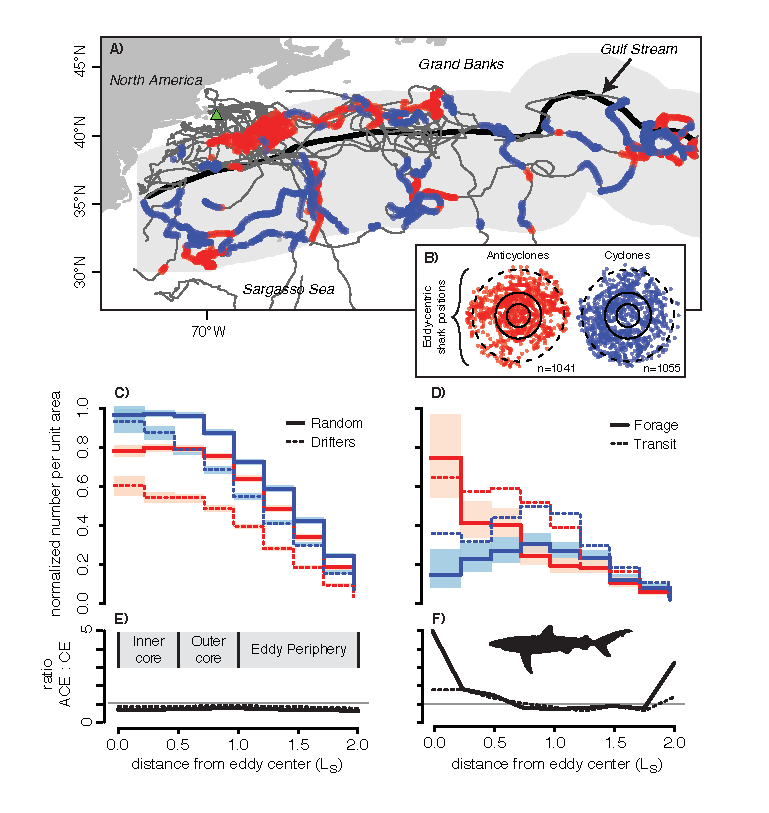
\includegraphics{images/C5_Fig1.pdf}
\caption[Use of Gulf Stream eddies by satellite-tagged blue sharks]{Blue sharks tagged in New England frequented the Gulf Stream eddy field (A) and occupied anticyclones (red throughout) and cyclones (blue throughout) at approximately the same frequency (B). Eddy-centric histograms indicated random walk simulations (solid, C) and passive drifters (dashed, C) exhibited higher cyclone use after controlling for eddy area. Sharks (D) used eddy peripheries ($>L_s$) approximately equally between eddies of either polarity, but more positions classified as "transiting" (dashed, D) were collocated around the eddy length scale ($L_s$) compared to "foraging" locations (solid, D). Sharks showed a marked preference for the cores of anticyclones relative to cyclones, particularly while foraging (D). The ratio of anticyclone (ACE) to cyclone (CE) positions across different regions of the eddies are shown for random walk simulations (E), drifters (E) and foraging (solid) and transiting (dashed) modes in the shark data (F). Note confidence intervals have been removed from the transit mode in panel D to aid visualization.}
\label{fig:c5f1}
\end{figure}
%-------------------------

%-------------------------
\clearpage
\begin{landscape}
\begin{table}
\caption[Tagging summary for SPOT and PSAT-tagged blue sharks in this study]{Tagging summary for SPOT and PSAT-tagged blue sharks in this study. SPOT TAL indicates time-at-liberty (in days) of the Argos-based SPOT tag data and SPOT per Day the average number of SPOT positions per day over the deployment. PSAT TAL indicates time-at-liberty for the PSAT tag. Track distance is cumulative trajectory distance (in km).}
\label{tab:c5t1}
\centering
%\begin{tabular}[t]{rllrrrlrlr}
\begin{tabular}{p{1.5cm} p{.8cm} p{2cm} p{1.5cm} p{1.5cm} p{1cm} p{1cm} p{1cm} p{1cm} p{2cm}}
\toprule
Shark ID & Tag Type & Tag Date & Tag Lat($^\circ$N) & Tag Lon($^\circ$W) & FL (cm) & SPOT TAL & SPOT per Day & PSAT TAL & Distance (km)\\
\midrule
106744 & SP & 2016-08-27 & 41.40 & 69.30 & 277 & 132 & 3.3 & 180 & 5,676\\
106745 & SP & 2016-08-28 & 41.52 & 69.43 & 270 & 131 & 4.5 & 180 & 5,587\\
106746 & SP & 2016-08-28 & 41.54 & 69.42 & 262 & 127 & 3.3 & 180 & 3,531\\
106747 & SP & 2016-10-18 & 41.47 & 69.33 & 295 & 74 & 4.3 & 172 & 3,501\\
106748 & SP & 2016-08-27 & 41.09 & 69.38 & 245 & 78 & 1.7 & DNR & 2,589\\
132346 & S & 2013-07-28 &  &  & 274 & 207 & 4.6 & NA  & 8,205\\
141195 & S & 2014-07-12 &  &  & 295 & 64 & 6.3 & NA & 2,280\\
141261 & SP & 2015-10-13 & 41.32 & 69.28 & 254 & 259 & 3.4 & 180 & 12,428\\
141262 & SP & 2016-08-28 & 41.54 & 69.42 & 221 & 131 & 3.0 & 121 & 5,686\\
141263 & SP & 2016-08-25 & 41.49 & 69.33 & 248 & 70 & 2.8 & 39 & 3,083\\
141264 & SP & 2015-10-21 & 41.59 & 69.45 & 254 & 158 & 4.8 & DNR & 6,253\\
141265 & SP & 2016-08-27 & 41.09 & 69.38 & 241 & 67 & 3.1 & 16 & 2,536\\
141266 & SP & 2016-09-10 & 41.75 & 69.83 & 254 & 77 & 3.4 & 112 & 4,221\\
141268 & SP & 2015-10-13 & 41.58 & 69.42 & 267 & 120 & 5.6 & 134 & 5,731\\
141270 & SP & 2015-10-21 & 41.60 & 69.44 & 274 & 288 & 6.7 & 107 & 14,485\\
165927 & SP & 2016-10-18 & 41.47 & 69.33 & 313 & 80 & 4.7 & DNR & 3,885\\
165928 & SP & 2016-10-18 & 41.47 & 69.33 & 290 & 54 & 3.8 & 127 & 3,034\\
\bottomrule
\end{tabular}
\end{table}
\end{landscape}
\clearpage
%-------------------------

\section{Results}

\subsection{Overall movements}

Blue sharks moved across a 25$^{\circ}$ and 40$^{\circ}$ latitudinal and longitudinal range, respectively, between highly dynamic Gulf Stream waters to oligotrophic, relatively homogeneous habitat in the Sargasso Sea. All 17 SPOT tags reported an average of 4 positions $\cdot$ day $^{-1}$ over 54-288 days at liberty (Table \ref{tab:c5t1}). Overall movements covered, on average, 5,454 km (2,280-14,485 km) in up to 288 days at liberty and were predominantly oriented east-west at temperate latitudes (Fig. \ref{fig:c5f1}). Depth and temperature data indicated blue sharks made extensive vertical movements offshore. Twelve PSAT tags deployed in this study reported and transmitted data, 7 of which reported >10 days early. The 12 reporting tags were at liberty for an average 129 days (range 16-180). PSAT-tagged sharks regularly dove to at least 400 m when offshore of the continental shelf (maximum depth 1,696 m), almost exclusively during daylight hours. Overall mean temperature occupied was 18.5$^\circ$C (range 3.9-31.8$^\circ$C), and blue sharks largely remained above the 10-12$^\circ$C isotherm while diving.

\subsection{Movements in the Gulf Stream eddy field}

Overall, 38\% of positions within the GS region were within cyclonic and anticyclonic eddies (19\% within eddies of each polarity; Fig. \ref{fig:c5f1}, Table \ref{tab:c5t2}). This represents similar use of eddies, based on frequency, to that indicated by CRW simulations (mean 20\% in CEs and 18\% in ACEs). However, individual variability in eddy use was high, and some individuals demonstrated highly significant use or avoidance of eddies. Percent frequency of positions collocated to eddies ranged from 2-39\% in ACEs and 4-28\% in CEs.

Blue shark locations in eddy-centric coordinates suggest qualitatively similar use of both eddy types (Fig. \ref{fig:c5f1}A, B); however, histograms of shark positions as a function of distance from eddy centers (normalized by the area of the annulus defined by each radial bin) revealed that blue sharks were significantly more likely to be associated with the inner-cores ($r \leq L_s / 2$) of ACEs than CEs, potentially driven by an avoidance of CE cores (Fig. \ref{fig:c5f1}C, E). Sharks were also significantly more likely to exhibit residency, rather than transiting, behavior while in ACE cores (Fig. \ref{fig:c5f1}C, E). In eddy peripheries, we observed no differences in overall use of eddies of either polarity. However, comparing collocated CRW simulations and drifter data suggests less use of ACE and CE peripheries ($r > L_s$) by sharks than by either null model (Fig. \ref{fig:c5f1}D, F). This is further corroborated by the behavior state data which indicates blue sharks were more likely to exhibit transit behavior near $L_s$ in eddies of either polarity. In fact, both drifters and CRW results suggested higher null "use" of CEs than ACEs which further supports active use of ACEs by blue sharks as they demonstrated equal or higher use of ACEs relative to CEs (Fig. \ref{fig:c5f1}).

%-------------------------
\begin{figure}[htbp]
\centering
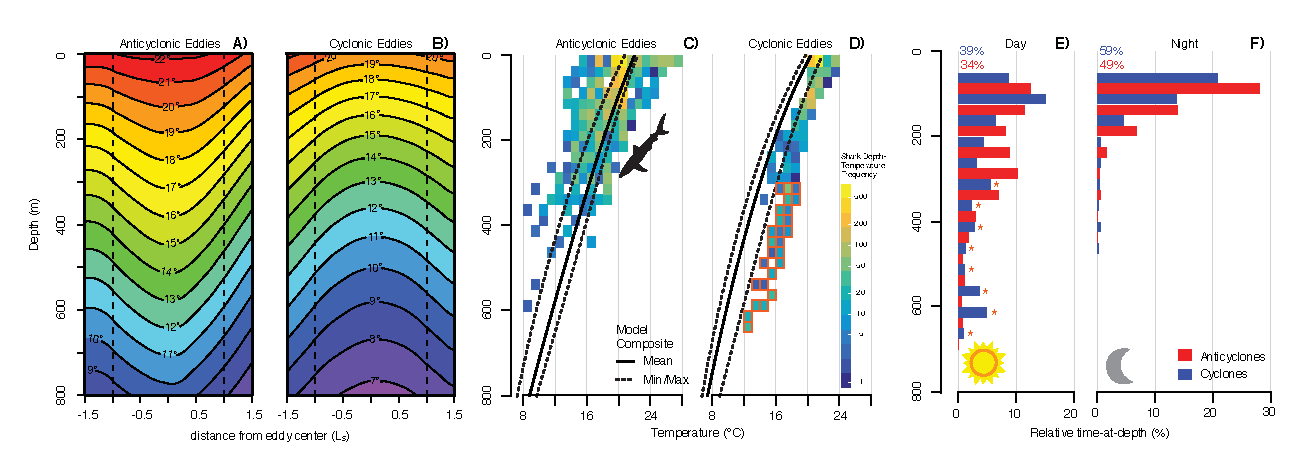
\includegraphics[width=\textwidth]{images/C5_Fig2.pdf}
\caption[Eddy vertical structure and blue shark diving]{Eddy vertical structure and blue shark diving. Modeled depth-temperature profile composites for 27 anticyclonic (A) and 28 cyclonic (B) eddies occupied by blue sharks. Histogram of blue shark depth-temperature data while diving in cores ($r < L_s$) of anticyclones (C; n=7,271) and cyclones (D; n=2,521) compared to model composite depth-temperature profiles. Summary of blue shark time-at-depth during day (E) and night (F) occupation of anticylonic (red) and cyclonic (blue) eddies. The 0-50m depth bin has been removed to aid visualization. The highlighted depth-temperature cells (orange outline, D) and time-at-depth bins (orange asterisks, E) correspond to diving in mode-2 cyclones.}
\label{fig:c5f2}
\end{figure}
%-------------------------

\subsection{Vertical structure of eddies and diving behavior}

HYCOM-derived composites for the shark-occupied eddies indicated eddy vertical structure typical of energetic Gulf Stream eddies. ACEs were characterized by warm surface water (22-23$^\circ$C) and depressed isotherms (Fig. \ref{fig:c5f2}A) resulting in positive (warm) temperature anomalies as high as 3$^\circ$C from 250-600 m (Fig. \ref{fig:c5f2}C). In contrast, CEs exhibited 19-20$^\circ$C SSTs with "domed" isotherms (Fig. \ref{fig:c5f2}B) and negative (cold) temperature anomalies >2$^\circ$C between 300-700 m (Fig. \ref{fig:c5f2}D).

Depth-temperature time series data derived from shark PSAT tags was collocated to eddies for a total of 15,189 depth measurements within eddy cores ($r \leq L_s$) at 2.5 minute resolution. When compared to eddy vertical composites, shark depth-temperature data from eddy cores were representative of these features in the Gulf Stream. Tagged individuals experienced a wide temperature range ($\pm$ 6$^\circ$C from mean ACE composite) while diving around the cores of ACEs (Fig. \ref{fig:c5f2}A) and a restricted range ($\pm$ 2$^\circ$C from mean CE composite) in CE cores (Fig. \ref{fig:c5f2}C). Blue sharks encountered positive temperature anomalies throughout their excursions below 150 m in ACEs, including warm anomalies as high as 10$^\circ$C from 250-350 m (Fig. \ref{fig:c5f2}C). In CEs, blue sharks occupied slightly warmer water than that predicted by HYCOM-derived composites (Fig. \ref{fig:c5f2}B). These features proved anomalously cold (-5$^\circ$C anomaly) in near-surface waters (Fig. \ref{fig:c5f2}C) but were otherwise within $\pm$ 2$^\circ$C of climatological mean temperatures at depth (Fig. \ref{fig:c5f2}D). 

Regardless of eddy polarity, tagged individuals spent 40-50\% of time in eddies in the upper 50 m of the water column and < 10\% of time while in eddies below 300 m. In general, tagged sharks spent more time-at-depth between 50-350 m in ACEs compared to CEs (Fig. \ref{fig:c5f2}); however, a small but notable increase in time-at-depth was observed deeper than 550 m in some Gulf Stream cyclones (Fig. \ref{fig:c5f2}). The limited deep diving (> 400 m) observed in ACEs occurred in typical warm core rings characterized by positive temperature anomalies at depth and temperatures > 12$^\circ$C at 600 m (Fig. \ref{fig:c5f3}). Diving in CEs was often shallower due to shoaling of isotherms (Fig. \ref{fig:c5f2}) resulting in compression of the available water column warmer than 10$^\circ$C (Fig. \ref{fig:c5f3}). Deep dives in CEs were constrained to those eddies that were low amplitude and/or old which made their vertical structure nearly indistinguishable from warm ambient water south of the GS (Fig. \ref{fig:c5f3}).

In addition to aggregate depth-temperature data, we extracted individual dives below 200 m in eddies. While the time series record contained 2.5x more dives below 200 m in ACEs compared to CEs, there was no significant difference in the depth or duration of dives between the two eddy types (Fig. \ref{fig:a5f1}).

%-------------------------
\begin{table}
\caption[Summary of anticyclonic and cyclonic eddy use by blue sharks in the Gulf Stream]{Summary of anticyclonic (ACE) and cyclonic (CE) eddy use by blue sharks in the Gulf Stream. Values represent frequency (Freq) and number (N) of positions in eddies of each polarity relative to total number of SPOT positions within the study area for each individual. Correlated random walk (CRW) values show frequency of eddy use by simulated random movements as mean mean (confidence interval). Asterisks (*) and crosses ($^{\dagger}$) indicate the observed eddy use by sharks is greater than and less than the confidence interval calculated from CRW simulations, respectively.}
\label{tab:c5t2}
\centering
\begin{tabular}[t]{ccccccc}
\toprule
 & \multicolumn{3}{c}{Anticyclonic Eddies} & \multicolumn{3}{c}{Cyclonic Eddies} \\
Tag ID & Freq & N & CRW & Freq & N & CRW\\
\midrule
106744 & 0.24* & 93 & 0.17 (0.15-0.19) & 0.28* & 108 & 0.23 (0.20-0.25)\\
106745 & 0.19* & 68 & 0.13 (0.12-0.15) &  & 0 & 0.20 (0.17-0.22)\\
106746 &  & 0 & 0.18 (0.15-0.22) & 0.28* & 33 & 0.11 (0.09-0.13)\\
106747 &  & 1 & 0.14 (0.12-0.16) & 0.07$^{\dagger}$ & 18 & 0.18 (0.16-0.21)\\
106748 & 0.33* & 36 & 0.15 (0.13-0.18) &  & 0 & 0.19 (0.15-0.22)\\
132346 & 0.20 & 21 & 0.20 (0.17-0.22) & 0.14$^{\dagger}$ & 15 & 0.19 (0.17-0.21)\\
141195 & 0.12$^{\dagger}$ & 20 & 0.15 (0.13-0.18) &  & 0 & 0.15 (0.13-0.18)\\
141261 & 0.21 & 160 & 0.23 (0.21-0.25) & 0.40* & 308 & 0.28 (0.26-0.3)\\
141262 & 0.20* & 93 & 0.14 (0.12-0.15) & 0.12$^{\dagger}$ & 55 & 0.21 (0.19-0.24)\\
141263 & 0.39* & 63 & 0.15 (0.12-0.18) & 0.17 & 28 & 0.17 (0.14-0.19)\\
141264 & 0.37* & 207 & 0.24 (0.21-0.26) & 0.24* & 138 & 0.21 (0.19-0.23)\\
141265 & 0.10$^{\dagger}$ & 16 & 0.15 (0.11-0.18) & 0.04$^{\dagger}$ & 7 & 0.17 (0.14-0.19)\\
141266 &  & 3 & 0.14 (0.12-0.16) & 0.20 & 18 & 0.21 (0.18-0.24)\\
141268 & 0.28* & 45 & 0.24 (0.21-0.26) & 0.18 & 30 & 0.18 (0.16-0.21)\\
141270 & 0.20 & 212 & 0.21 (0.19-0.23) & 0.25$^{\dagger}$ & 259 & 0.28 (0.27-0.3)\\
165927 & 0.02 & 6 & 0.16 (0.14-0.19) & 0.14$^{\dagger}$ & 35 & 0.23 (0.20-0.26)\\
165928 & 0.15 & 23 & 0.16 (0.14-0.19) & 0.08$^{\dagger}$ & 12 & 0.16 (0.12-0.20)\\
ALL & 0.19* & 67 & 0.18 (0.17-0.18) & 0.19$^{\dagger}$ & 76 & 0.20 (0.20-0.21)\\
\bottomrule
\end{tabular}
\end{table}
%-------------------------

\section{Discussion}

Meso- and submesoscale dynamics structure ocean ecosystems and generate patchiness that is fundamental to ocean ecology \citep{McGillicuddy2016, Mahadevan2016}. Yet, how these physical-biological interactions influence pelagic fish communities remains poorly understood. Our results identify mesoscale eddies as key drivers of movements and behavior of a model pelagic predator, the blue shark.

Blue sharks in our study exhibited wide-ranging and highly variable movements despite study individuals being primarily from the same demographic and tagging location. These data broadly fit with results from other tagging efforts in the Atlantic which report widespread pelagic movements of blue sharks outside of coastal aggregation periods \citep{Vandeperre2014, Campana2011, Howey2017}. Previous work has suggested the importance of the Gulf Stream as overwintering habitat for immature individuals \citep{Campana2011} and as a conveyor for females (most of which have recently mated) moving offshore and some toward the eastern Atlantic \citep[reviewed in][]{Nakano2008}. All individuals in our study were mature males that occupied the Gulf Stream region during winter months, further corroborating its role as overwintering habitat for this species.

\subsection{Mesoscale dynamics of the Gulf Stream and the role of eddies}

% role of ACEs relative to CEs
The Gulf Stream is one of the most dynamic regions of the world ocean and contains some of the most highly energetic eddies on earth \citep{Chelton2011}. These features can have significant impacts on pelagic communities \citep{Gaube2017DSR} and ecosystem dynamics \citep{Davis1985, Boyd1986, Gaube2018}. Our eddy collocation analysis demonstrated the role of eddies in driving blue shark movements and behavior in the Gulf Stream. Overall, our results suggest preferential occupation of the cores of ACEs. Similar results have been shown for white sharks in the Gulf Stream \citep{Gaube2018}, southern bluefin tuna in Australia \citep{Hobday2014} and turtles in the Bay of Biscay \citep{Doyle2008}, Brazil-Malvinas confluence \citep{Gaube2017} and off the southeastern coast of Africa \citep{Luschi2003}. All of these studies suggest higher use of ACEs is likely due, at least in part, to elevated foraging opportunities. However, others have proposed thermoregulatory \citep{Campana2011, Gaube2018, Gaube2017} and navigational functions \citep{Carey1990}.

%-------------------------
\begin{figure}[htbp]
\centering
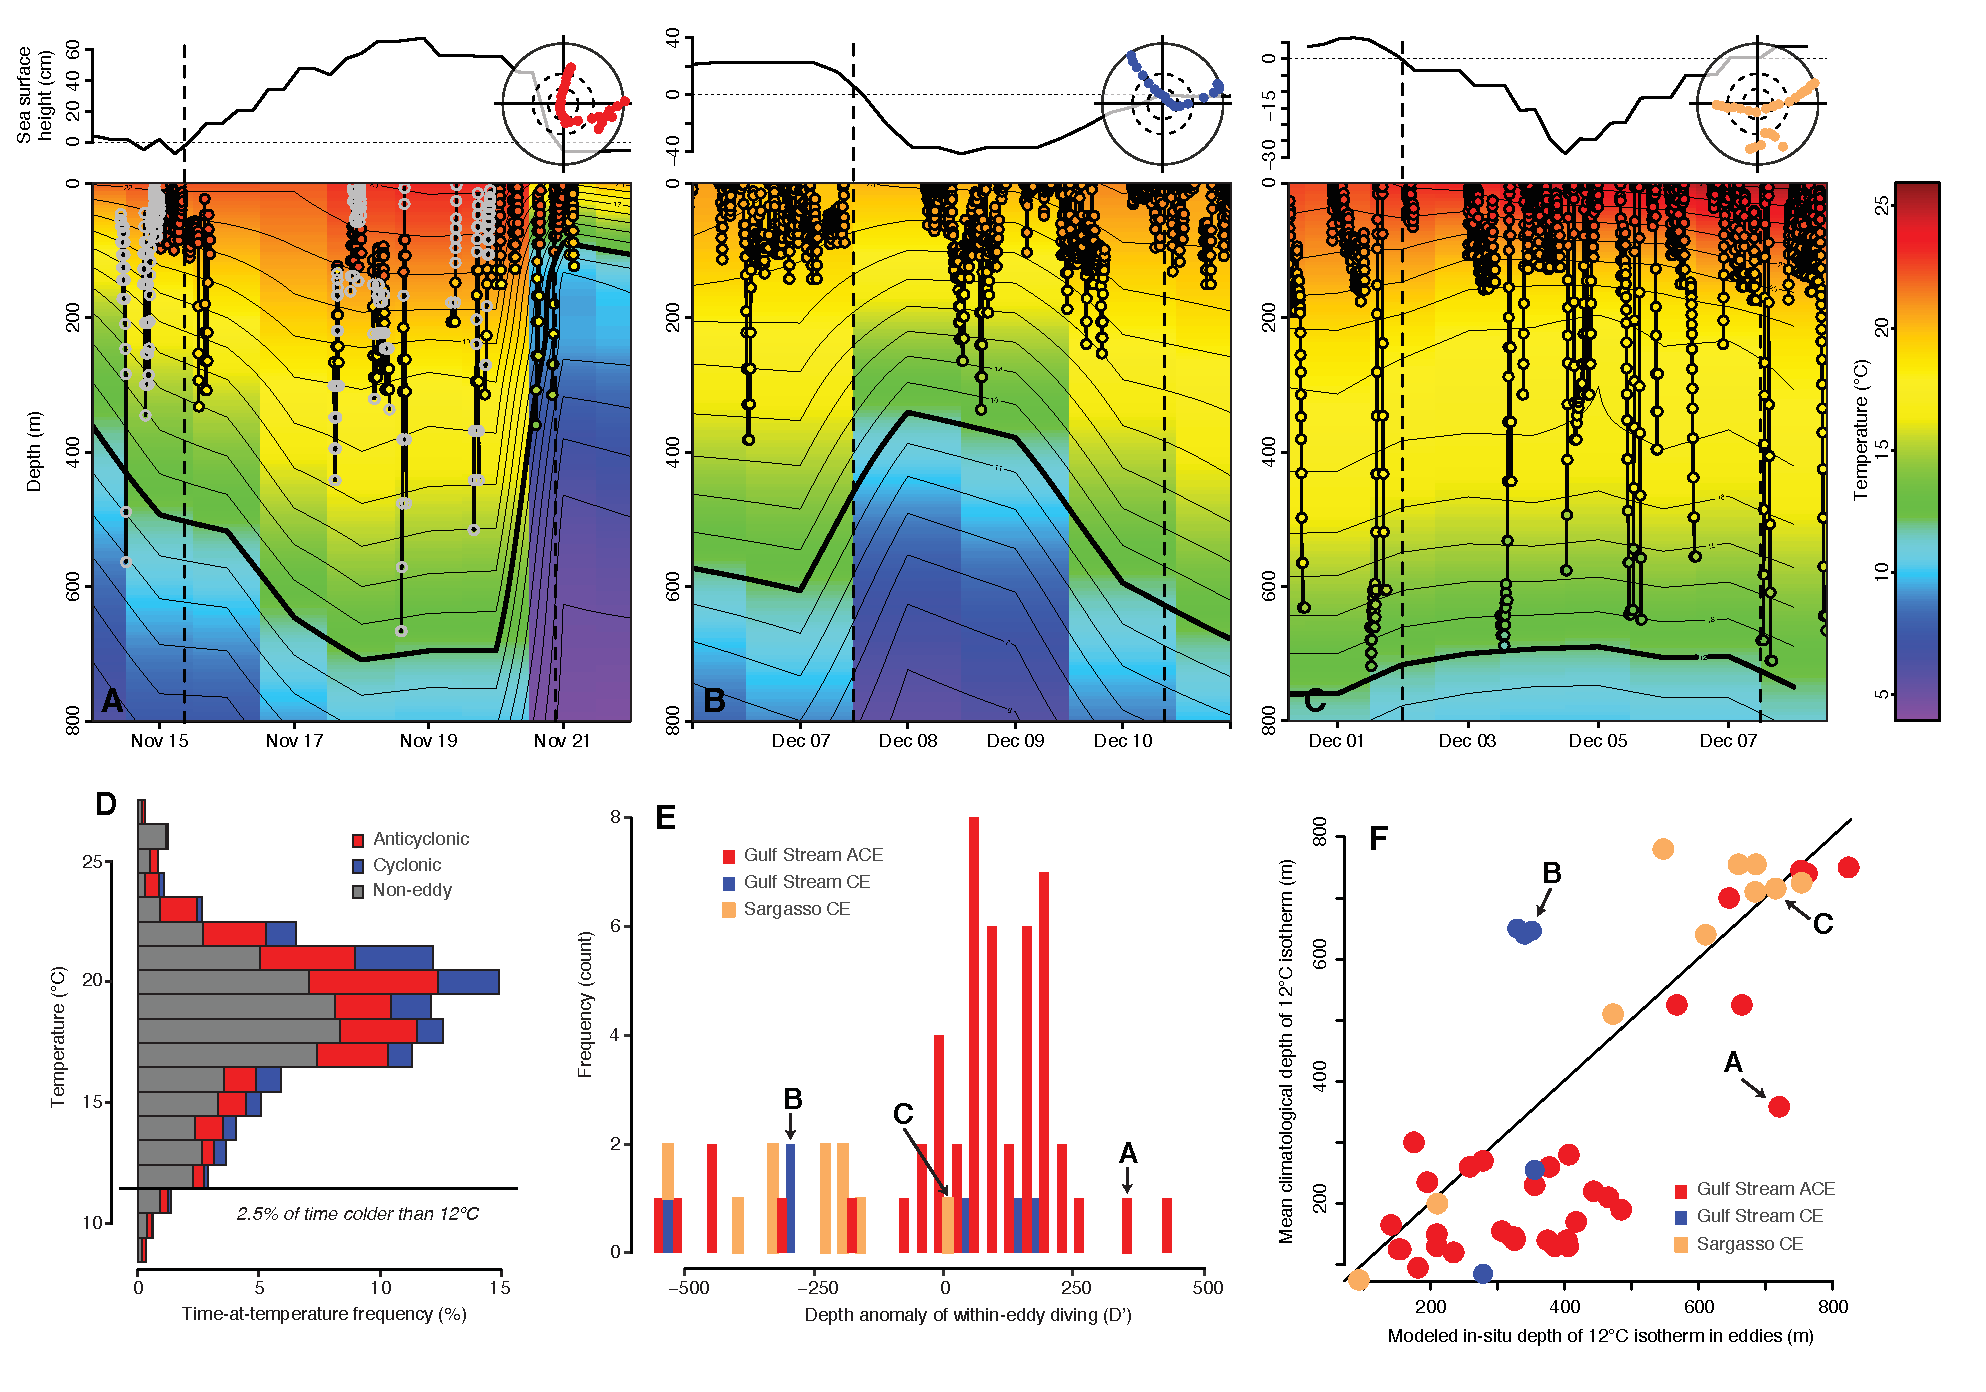
\includegraphics[width=\textwidth]{images/C5_Fig3.pdf}
\caption[Example diving by blue sharks in Gulf Stream eddies and a Sargasso Sea cyclone]{Example diving by blue sharks in anticyclonic (A) and cyclonic (B) Gulf Stream eddies and a cyclonic eddy of Sargasso Sea origin (C). Upper line plots indicate measured sea surface height from AVISO (Eqn. \ref{eq:ssh}). Top right circular plots in each panel show geographic movements of the shark in eddy-centric coordinates (as in Fig. \ref{fig:c5f1}). Water column structure in the eddies (color map, top panels) is modeled depth-temperature data from HYCOM. Colored points connected by solid vertical lines represent shark diving behavior (grey circles indicate no temperature data was acquired/transmitted by the tag for a given depth point in the time series). Dashed vertical lines indicate entry and exit of eddies based on SSH. Thin, labeled horizontal lines indicate isotherms at 1$^\circ$C intervals. Frequency histogram of the time-at-temperature distribution for all shark dive data in the Gulf Stream (D) and for the depth anomaly of within-eddy diving (E; see Eq. \ref{eq:dprime}). Positive $D'$ indicates sharks dove below the climatological 12$^\circ$C isotherm, suggesting vertical downward displacement of isotherms by the eddy as shown by comparing climatological mean isotherm depth to \is modeled isotherm depth within eddies (F).}
\label{fig:c5f3}
\end{figure}
%-------------------------

%\subsection{Potential mechanisms driving eddy use}
% why ACEs: 3 explanations, foraging thermoregulation navigation

%% thermo
Our results suggest two, likely interacting, explanations for the observed eddy use based on foraging and thermoregulation. Sharks in our study regularly conducted diel vertical migration while offshore from the surface during night to periods of regular dives into the mesopelagic (200-400 m) during daytime. These results are consistent with previous studies tracking blue sharks in the Gulf Stream that also reported a high frequency of octopods, a diel vertical migrator that occurs principally below 250 m, in blue shark stomachs \citep{Carey1990}. Thus, these deep dives may be associated with foraging for cephalopods, one of the blue sharks primary prey items \citep{Clarke1974, Henderson2001}, that are known to concentrate at depth particularly along the Gulf Stream front \citep{Vovk1978, Fedulov1986, Dawe1985}. 

While these data suggest Gulf Stream-wide foraging in the mesopelagic, our collocation analysis indicated a significantly higher number of positions were recorded in the cores of ACEs than CEs in the Gulf Stream, a trend that was further pronounced when considering shark positions separately based on transiting or resident behavior state. We observed sharks more often exhibited residency in ACE cores which may be indicative of foraging \citep{Breed2009} in these features. While ACEs are typically characterized by low productivity and CEs more often contain enhanced chlorophyll and phytoplankton biomass \citep{Gaube2017DSR}, some ACEs have been observed containing enhanced productivity in their cores during winter \citep{Dufois2016}. In fact, \cite{Fennell2015} found enhanced mesopelagic backscatter in North Atlantic ACEs near the Grand Banks where they measured DSL densities that were comparable to the highest average (integrated from 200-1000 m) densities in the world oceans. \cite{Fennell2015} also found a positive correlation between backscatter and temperature at 400-600 m and observed observed extensive backscatter below 100-200 m in these features. Blue sharks in our study regularly dove > 200 m (and as deep as 700 m) in ACEs where these individuals experienced the strongest positive temperature anomaly measured in this region.

Previous studies have suggested the thermoregulatory implications of mesopelagic diving. \citep{Carey1990} fitted a blue shark with a cranial thermistor which indicated thermal hysteresis allowed this individual to maintain body temperatures that were significantly above (average +4$^\circ$C) ambient water temperatures as cold at 8$^\circ$C at 300 m. When muscle cooled to ~15$^\circ$C, the shark aborted the dive and returned to the surface to regain heat loss until muscle temperatures recovered to near 20$^\circ$C before repeating the dive-surfacing cycle. We observed similar oscillatory diving into the mesopelagic during daytime in both types of Gulf Stream eddies that was seemingly constrained by temperature at depth (Fig. \ref{fig:c5f3}), consistent with the behavioral thermoregulation observed by \cite{Carey1990}. Sharks spent more time shallower than 50 m in CEs while the time-at-depth distribution was shifted deeper in ACEs (Fig. \ref{fig:c5f2}). Blue sharks diving in ACEs spent considerable time-at-depth, regularly as deep as 300-350 m, where backscatter is likely high \citep{Fennell2015} and temperatures were consistently >12$^\circ$C. Thus, it seems the potentially enhanced foraging opportunities combined with relaxing of thermal constraints in ACEs may interact to drive blue shark preference for these features.

\section{Conclusion}

Current management approaches largely ignore (sub)mesoscale ocean dynamics that dominate open ocean heterogeneity and discount the multitude of physical-biological interactions at and below the mesoscale as static phenomena \citep{Maxwell2015, Lewison2015}. Yet, we demonstrate clear links between mesoscale physical dynamics of the Gulf Stream region and movements and behavior of a model predator, the blue shark, using combined animal telemetry and a multi-satellite analysis framework. Our data suggest blue sharks may be targeting anticyclonic eddies in the Gulf Stream, which have been deemed "buses of productivity" \citep{Fennell2015}, where enhanced foraging opportunities co-occur with anomalously warm water at depth, providing particularly suitable overwinter habitat for this species. 

Future work should seek to directly link observed behaviors with foraging. Interspecific comparisons, particularly with other predator species across the spectrum of highly endothermic (\eg shortfin mako) to fully ectothermic (\eg tiger shark) could provide additional insight on the thermoregulatory role and physiological implications of these features. Comparative studies across similarly dynamic regions such as the Agulhas and less dynamic, but eddy-rich areas such as the Sargasso Sea should provide additional inference on the role of mesoscale eddies in structuring pelagic ecosystems. 

